% !TEX spellcheck = en_US
% Tower Damper
%=================================================================================
This section describes the the function and the implementation of a pitch angle based Tower Damper (TD). !!! Abbreviation package !!! The design follows the description in \cite{WindEnergyHandbook} similar as the workflow in the exercise of the corresponding lecture and lecture notes \cite{2024}. The tower dynamics are modeled as in \cite{WindEnergyHandbook} (eq: 8.12 and 8.13). Here referd as \ref{eq:TowerDynamics} and \ref{eq:TowerDamper}.
\begin{equation}
	M\ddot{x} + D\dot{x} + Kx = F + \Delta F
	\label{eq:TowerDynamics}
\end{equation}
\begin{equation}
	\begin{aligned}
		\Delta F = \frac{\partial F}{\partial \theta}\Delta\theta = -D_{\text{TD}}\dot{x}\\
		\Delta\theta = \frac{-D_{\text{TD}}}{\partial F/\partial \theta}\dot{x}
	\end{aligned}
	\label{eq:TowerDamper}
\end{equation}
As described by equation \ref{eq:TowerDynamics} the dynamics of the tower in fore-aft direction are lightly damped if $D$ is small and the force $\Delta F$ which is the additional thrust force resulting of a pitch action is equal to zero. The force $F$ is damped by the relative wind speed $v_{\text{rel}} = v_0 - \dot{x}$ and therefore $F = F(\Omega, \theta, v_{\text{rel}})$ \cite{2024}. To damp the tower top speed $\dot{x}$ even further \cite{WindEnergyHandbook} proposes an update of the pitch angle of $\Delta\theta$. This will damp the tower motion further as described in \ref{eq:TowerDamper}. This lead to a reduction of the tower bottom bending moment. Nevertheless this comes at a cost of higher pitch activity and the damping is only available in control region 3. The static tower top deflection over the regions are shown in section \ref{steady states}. This is helpful to see when the damper is active and what can be damped. 

The implementation and test of the damper is done in Matlab and Simulink. As in the lecture and the corresponding exercise \cite{2024} the tower top acceleration $\ddot{x}$ is measured in reality. To make the simulation task as similar to a real world application here also the the tower top acceleration is used. What is also taken into account is the existence of a real pitch actuator. This means that the pitch update $\Delta\theta$ can not be applied instantaneously because of the time constants of the pitch actuator. To address this phenomena there are 2 methods tested. First a direct integration \ref{eq:TDintegration}: 
\begin{equation}
	\dot{x}(t) = \int\ddot{x}(t) \text{d}t
	\label{eq:TDintegration}
\end{equation} 
And second a phase shift of $90^{\circ}$ of the speed signal by a Lag-Compensator. The Transferfunction in the frequency domain is shown in equation \ref{eq:LagCompensator}. Where the input in the frequency domain is $\ddot{X}$ and the output is $\dot{X}$. 
\begin{equation}
	\frac{\ddot{X}(s)}{\dot{X}(s)} = \frac{s + z}{s + p}
	\label{eq:LagCompensator}
\end{equation} 
\begin{equation}
	\dot{x}(t) = \ddot{x}(t) - \int p\dot{x}(t) - z\ddot{x}(t) \text{d}t
	\label{eq:xddTimeDomain}
\end{equation} 

% explain analytical why this should work better

The implementation in Simulink is first following the approach in the exercise \cite{2024}.
\begin{figure}[tbh]
	\centering	
	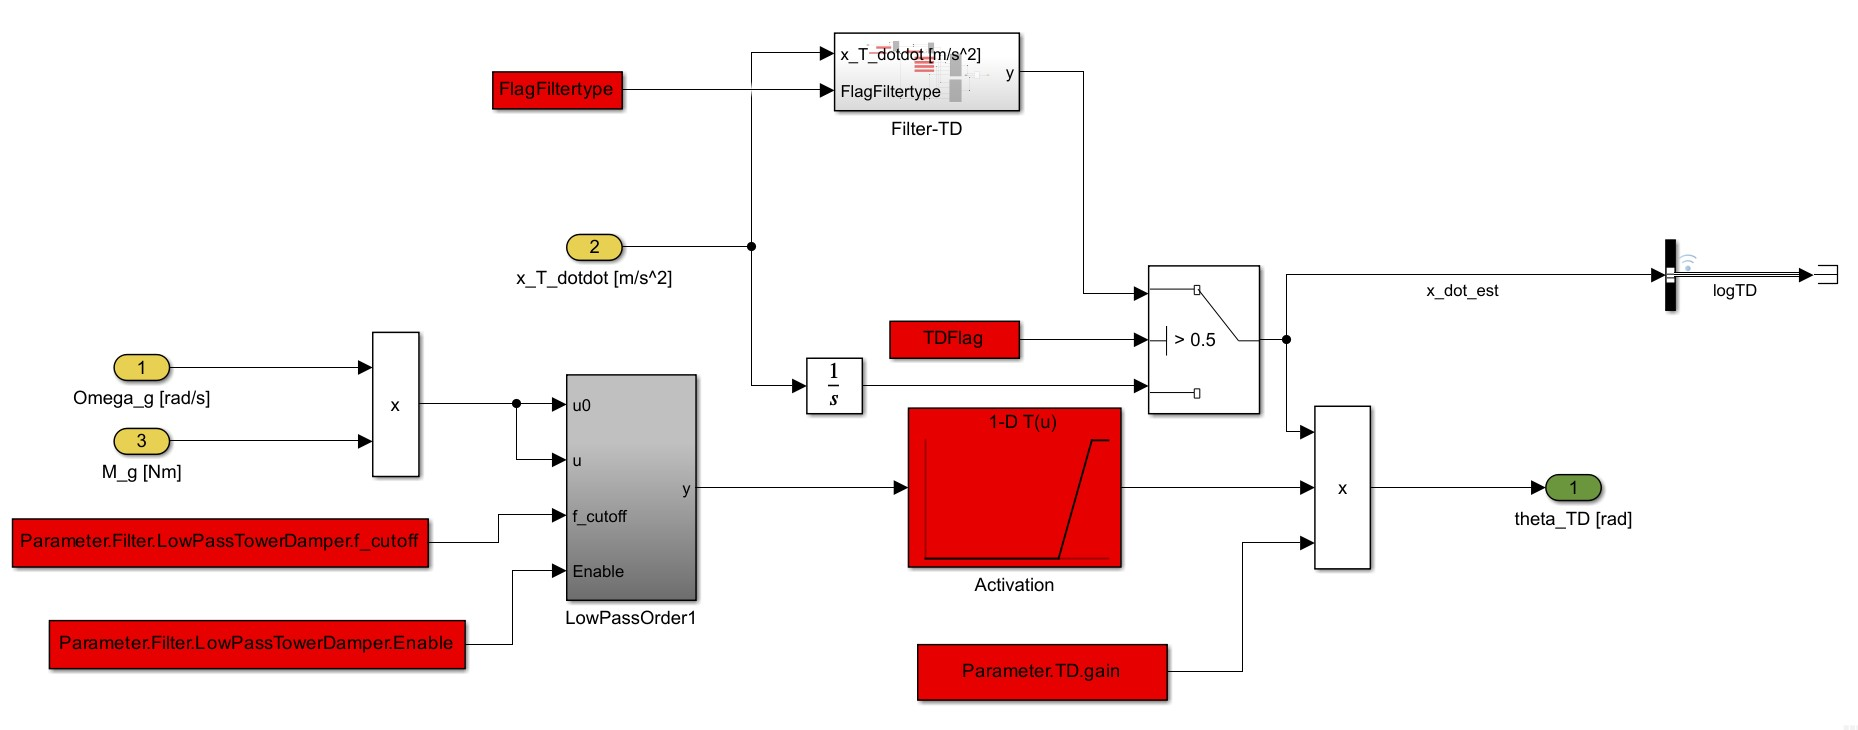
\includegraphics[width=12cm]{Figures/TDoverview}
	\caption{Tower Damper in Simulink model}
	\label{fig:TDoverview}
\end{figure}  
The input \textit{Omega\_g} is already a filtered value. It is low pass filtered and the 3P blade passing frequency is notched. As shown in figure \ref{fig:TDoverview} to activate the TD the generator power is used. The \textit{LowPassOrder1} is used to reduce the switching frequency of the TD to ensure that it is not switched on and of if the WT is operating near rated conditions. In the activation the gain is slowly ramped up from $\SI{0}{\%}$ to $\SI{100}{\%}$ over a power range from $\SI{80}{\%}$ of the rated power to $\SI{100}{\%}$ and stays there. 